\documentclass[smaller,usepdftitle=false]{beamer}
\usepackage[latin1,utf8]{inputenc}
\usepackage[T1]{fontenc}
\usepackage{tikz}
\usetikzlibrary{topaths}


\mode<presentation>
\usetheme{Warsaw}
\setbeamertemplate{navigation symbols}{}
\setbeamertemplate{headline}{}
\setbeamertemplate{footline}{}
%\usecolortheme{beetle}
\usepackage[matrix,arrow,graph,curve]{xy}
\usepackage{amssymb}
\usepackage{leftidx}
\usepackage{graphics}
\usepackage{cancel}
\usepackage{xcolor}

\newcommand\NN{\mathbb N}
\newcommand\CC{\mathbb C}
\newcommand\QQ{\mathbb Q}
\newcommand\RR{\mathbb R}
\newcommand\ZZ{\mathbb Z}

\newcommand\maps{\longmapsto}
\newcommand\ot{\otimes}
\renewcommand\to{\longrightarrow}
\renewcommand\phi{\varphi}
\newcommand\stack[2]{\genfrac{}{}{0pt}{2}{#1}{#2}}
\newcommand\vectspan[1]{\left\langle #1 \right\rangle}

%%%%%%%%%%%%%%%%%%%%%%%%% Specific notation %%%%%%%%%%%%%%%%%%%%%%%%%
\newcommand\A{\mathcal A}
\newcommand\B{\mathcal B}
\newcommand\C{\mathcal C}
\newcommand\D{\mathcal D}
\newcommand\I{\mathcal I}
\renewcommand\S{\mathcal S}
\newcommand\K{\mathcal K}
\newcommand\F{\mathcal F}
\newcommand\G{\mathcal G}
\newcommand\GG{\Gamma}
\renewcommand\L{\mathcal L}
\newcommand\M{\mathcal M}
\renewcommand\O{\mathcal O}
\newcommand\R{\mathcal R}
\newcommand\tphi{\tilde \phi}
\renewcommand\a{\mathfrak a}
\renewcommand\b{\mathfrak b}
\newcommand\q{\mathbf{q}}
\newcommand\m{\mathfrak m}
\newcommand\n{\mathfrak n}
\newcommand\g{\mathfrak g}
\newcommand{\Rho}{\mathrm{P}}
\newcommand\opp{\circ}
\newcommand\norm{\mathsf{norm}}
\newcommand\join{\vee}
\newcommand\meet{\wedge}
\newcommand\DC{\mathsf{DC}}

\DeclareMathOperator\Ab{\mathsf{Ab}}
\DeclareMathOperator\Vect{\mathsf{Vect}}

\newcommand\SET{\textsf{SET}}
\newcommand\set{\textsf{set}}
\newcommand\Set{\textsf{Set}}


\DeclareMathOperator\mmod{\mathsf{mod}}
\DeclareMathOperator\Sgrp{\mathsf{Sgrp}}
\DeclareMathOperator\Grp{\mathsf{Grp}}
\DeclareMathOperator\CoMod{\mathsf{CoMod}}

\DeclareMathOperator\Mod{\mathsf{Mod}}
\DeclareMathOperator\Hom{\mathsf{Hom}}
\DeclareMathOperator\Ext{\mathsf{Ext}}
\DeclareMathOperator\Tor{\mathsf{Tor}}

\DeclareMathOperator\GrMod{\mathsf{GrMod}}
\DeclareMathOperator\grmod{\mathsf{grmod}}
\DeclareMathOperator\GrHom{\underline{\mathsf{Hom}}}
\DeclareMathOperator\GrExt{\underline{\mathsf{Ext}}}
\DeclareMathOperator\GrTor{\underline{\mathsf{Tor}}}

\DeclareMathOperator\im{Im}
\DeclareMathOperator\id{injdim}
\DeclareMathOperator\pd{pdim}
\DeclareMathOperator\gr{\mathsf{gr}}
\DeclareMathOperator\ldim{ldim}
\DeclareMathOperator\height{\mathsf{ht}}
\DeclareMathOperator\st{\mathsf{st}}
\DeclareMathOperator\depth{depth}
\DeclareMathOperator\lcd{lcd}
\DeclareMathOperator\lex{\mathsf{lex}}
\DeclareMathOperator\Spec{Spec}
\DeclareMathOperator\supp{supp}
\DeclareMathOperator\Id{Id}
\DeclareMathOperator\rank{rk}
\DeclareMathOperator\rk{rk}
\DeclareMathOperator\irr{irr}
\DeclareMathOperator\GKdim{\mathsf{GKdim}}
\DeclareMathOperator\relint{\mathsf{relint}}
\DeclareMathOperator\coker{\mathsf{coker}}
\DeclareMathOperator\tr{\mathsf{tr}}
\DeclareMathOperator\SL{\mathsf{SL}}
\DeclareMathOperator\ev{\mathsf{ev}}

\def\pausa{\pause \bigskip}



\title[]{Charlas UBACs: La geometr\'ia del SET}
\author[]{Pablo Zadunaisky Bustillos}
\date{Mayo 2014 2014}

\begin{document}
% Remove this to get the pauses...
\let\pause\relax
\begin{frame}
\titlepage
\end{frame}

\begin{frame}
\frametitle{Cartas de SET}
\begin{figure}[h!]
\centering
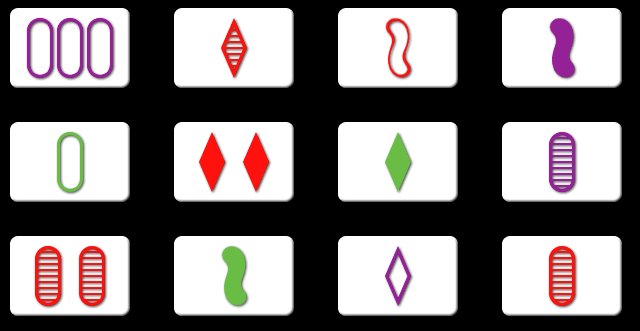
\includegraphics[width=0.8\textwidth]{cards2}
\end{figure}
\end{frame}

\begin{frame}
Las cartas tienen cuatro atributos, cada uno en tres variantes posibles:
\begin{table}
\centering
\begin{tabular}{|c |c|}
\hline
Numero: & 1, 2 o 3.  \\
\hline
Forma: & Diamante, fideo u óvalo.\\
\hline
Color: &Verde, celeste o fucsia.\\
\hline
Relleno: &Vacío, rayado o lleno.\\
\hline
\end{tabular}
\end{table}
\pause

Un \SET~es una familia de tres cartas que cumplen con lo siguiente: \textbf{Las
tres cartas son todas iguales o todas distintas para cada atributo}. 
\end{frame}

\begin{frame}
\frametitle{Por ejemplo}
\begin{figure}[h!]
\centering
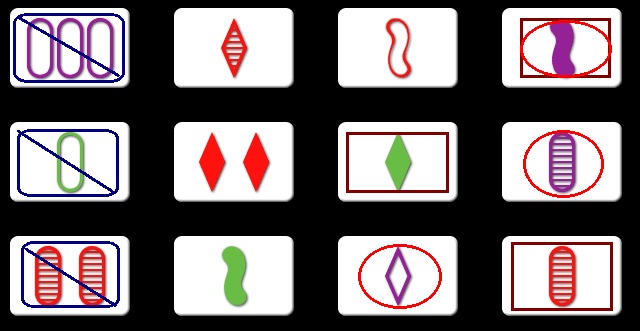
\includegraphics[width=0.8\textwidth]{cards3}
\end{figure}
\end{frame}
\begin{frame}{Datos...}
\begin{itemize}
\item Hay exactamente una carta con cada combinación posible de todos los atributos, así
que hay $3^4 = 81$ cartas en el mazo del \SET.

\item Dadas dos cartas, hay exactamente una carta con la que forman un \SET.

\item Hay exactamente $\frac{1}{3}\binom{81}{2} = 1080$ \SET's distintos.

\item Cada carta aparece en exactamente 40 \SET's.
\end{itemize}
\end{frame}

\begin{frame}
\frametitle{Pregunta:}
\noindent \textbf{¿Cuántas cartas hay que poner sobre la mesa para estar
seguro de que aparece un \SET~entre ellas?} 

\pause

¡Más de veinte!

\begin{figure}[h!]
\centering
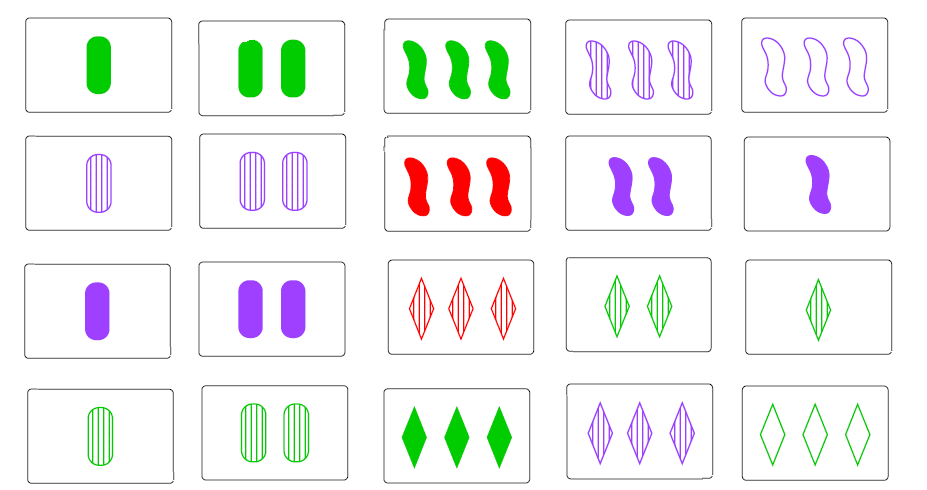
\includegraphics[width=0.85\textwidth]{caps}
\caption{Veinte cartas sin un \SET.}
\end{figure}
\end{frame}

\begin{frame}
\frametitle{Un juego más sencillo: el \set}

\begin{figure}[h!]
\centering
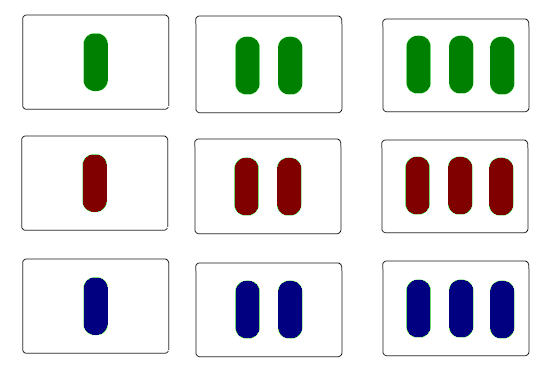
\includegraphics[width=0.85\textwidth]{ov-rojo}
\caption{Cartas de \set.}
\end{figure}
\end{frame}

\begin{frame}
\frametitle{Un juego más sencillo: el \set}

\begin{figure}[h!]
\centering
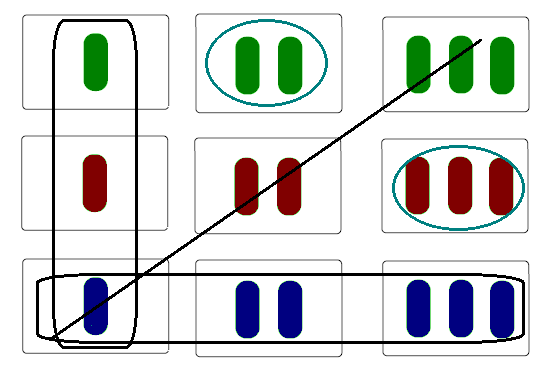
\includegraphics[width=0.85\textwidth]{ov-rojo-s}
\caption{\set's.}
\end{figure}
\end{frame}

\end{document}


